\chapter{Sistemi di telecomunicazione su canale passa banda}\label{cap:sis_telcom_band_pass}
\section{Introduzione}
Nei sistemi di trasmissione su canale radio è necessario tener conto delle caratteristiche di risposta in frequenza del mezzo trasmissivo: lo spettro in una banda di frequenze che si può allocare, in generale, è diverso da quello del segnale che si vuole trasmettere. Per abilitare la comunicazione è pertanto necessario traslare la banda del segnale originario per adattarsi alla banda di frequenze permesse dal mezzo trasmissivo, che ha funzione di trasferimento tipica di un filtro passa banda.

Questo tipo di canali si comportano in modo soddisfacente quando la frequenza relativa $f_r=\frac{f_0}{B}$ è sufficientemente piccola. Tale requisito è necessario ad alte frequenze per limitare la risposta tempovariante che si riduce operando in banda stretta.

I segnali che possono essere trasmessi su questo tipo di canali sono sinusoidi o somma di sinusoidi. L'informazione è contenuta nell'ampiezza del segnale e nella sua fase.

\clearpage
\section{Modulazione di ampiezza}
\[s_t(t)=s(t)\cdot\cos{\omega_0 t}\]
\section{In doppia banda laterale e portante soppressa (DSB-SC)}
\section{Demodulazione coerente (DSB-SC)}
\section{Modulazione d'ampiezza con portanti in quadratura}
\section{Effetto di un filtro frapposto tra modulatore e demodulatore}
\section{Rapporto Segnale Rumore (DSB-SC)}
\section{Modulazione d'ampiezza in banda laterale unica (SSB)}
\section{Modulatore SSB con filtraggio}
\section{Demodulazione SSB}
\section{Modulazione d'ampiezza con portante trasmessa}

\clearpage
\section{Modulazione angolare}
Nella modulazione d'ampiezza sono necessari amplificatori lineari: lo stadio di trasmissione è poco efficiente. Per questo motivo si introduce la \keyword[modulazione!angolare]{modulazione angolare} in cui l'informazione del segnale modulante è codificata nella fase (eq.\ref{eq:modulazione_fase}) o nella frequenza (eq.\ref{eq:modulazione_frequenza}).

Il \textsc{segnale trasmesso} ha formulazione non lineare \[s_T(t)=A\cos{\Phi(t)}\] e si può avere \keyword[modulazione!di fase]{modulazione di fase}
\begin{equation}s_T(t)=A_p \cos{\omega_0 t + \phi(t)}\label{eq:modulazione_fase}\end{equation}
e \keyword[modulazione!di frequenza]{modulazione di frequenza}
\begin{equation}s_T(t)=A_p \cos{\omega(t) t + \phi}\label{eq:modulazione_frequenza}\end{equation}

Il segnale trasmesso passa banda può essere rappresentato nelle sue componenti in fase e quadratura come nella modulazione di ampiezza:
\begin{equation}
s_T(t)=s_T^\text{I}(t)\cos{\omega_0 t}-s_T^\text{Q}(t)\sen{\omega_0 t}
\end{equation}
Nella modulazione angolare con portante a frequenza $f_0=\omega_0/2\pi$:
\begin{equation}\begin{split}
s_T(t)&=A_T(t)\cos{\omega_0 t+\phi_T(t)}=\\&=A_T(t)\cos{\omega_0 t}\cos{\phi_T(t)}-A_T(t)\sen{\omega_0 t}\sen{\phi_T(t)}
\end{split}\end{equation}
dove
\begin{equation}
\begin{cases}
s_T^\text{I}(t)=A_T(t)\cos{\phi_T(t)}\\s_T^\text{Q}(t)=A_T(t)\sen{\phi_T(t)}
\end{cases}\iff\begin{cases}
A_T(t)=\sqrt{{s_T^\text{\small I}}^2(t)+{s_T^\text{Q}}^2(t)}\\\phi_T(t)=\arctan\frac{s_T^\text{Q}(t)}{s_T^\text{I}(t)}
\end{cases}
\end{equation}

\begin{definizione}Si definiscono la \keyword[pulsazione!istantanea]{pulsazione istantanea}\begin{equation}\omega_i(t)=\deriv{\Phi(t)}{t}= \omega_0+\deriv{\phi(t)}{t}\end{equation} e la \keyword[pulsazione!deviazione di]{deviazione di pulsazione}\begin{equation}\Delta\omega(t)=\omega_i(t)-\omega_0
\end{equation}\end{definizione}
\begin{definizione}Si definiscono la \keyword[frequenza!istantanea]{frequenza istantanea}\begin{equation}f_i(t)=\frac{1}{2\pi}\omega_i(t)=f_0+\frac{1}{2\pi}\deriv{\phi(t)}{t}=f_0+\Delta f(t)\end{equation} e \keyword[frequenza!deviazione di]{deviazione di frequenza}\begin{equation}\Delta f(t)=\frac{\dot{\phi}(t)}{2\pi}\end{equation}\end{definizione}

\begin{nota}
La fase e la frequenza si possono determinare contando gli attraversamenti dell'asse dei tempi, rilevando i cambi di segno del segnale. La tecnica di modulazione angolare è robusta alle distorsioni sull'ampiezza introdotte da amplificatori non lineari.
\end{nota}

Il segnale ricevuto su canale passa banda può sempre essere espresso nelle sue componenti in fase e quadratura:
\begin{equation}\begin{split}
s_R(t)&=k s_T^\text{I}(t-T_g)\cos{\omega_0(t-T_f)}+\\
&+k s_T^\text{Q}(t-T_g)\cos{\omega_0(t-T_f)}
\end{split}\end{equation}
dove il fattore $k$ tiene conto dell'attenuazione del canale, $T_g$ è il ritardo di gruppo, $T_f$ il ritardo di fase.

In particolare per la modulazione angolare il segnale ricevuto con le sue portanti in fase e quadratura
\begin{equation}\begin{split}
s_R(t)&=S_T^\text{I}(t)\cos{\omega_0 t}-S_T^\text{Q}(t)\sen{\omega_0 t}=\\&=A_R(t)\cos{\omega_0 t+\phi_R(t)}
\end{split}\end{equation}

Al segnale ricevuto si somma il rumore, variabile aleatoria con distribuzione uniforme, si può esprimere nelle componenti in fase e quadratura:
\begin{equation}
N_T(t)=n^\text{I}(t)\cos{\omega_0 t}-n^\text{Q}(t)\sen{\omega_0 t}=\rho(t)\cos{\omega_0 t+\phi_n(t)}
\end{equation}

Nella modulazione angolare si riceve pertanto la somma dei segnali esprimibili in notazione fasoriale
\begin{equation}\begin{split}
&A_R(t)\cos{\omega_0 t+\phi_R(t)}+\rho(t)\cos{\omega_0 t+\phi_n(t)}=\\
&=\Re{A_R\e{\jmath\phi_R(t)}\e{\jmath\omega_0 t}+\rho(t)\e{\jmath\omega_0 t}\e{\phi_n(t)}}=\\
&=\Re{\rho(t)\e{\jmath(\phi_R(t)+\beta(t))}}
\end{split}\end{equation}

\section{Spettro di una sinusoide modulata angolarmente}
La non linearità della modulazione angolare non consente il calcolo dello spettro della portante modulata per un segnale qualsiasi. La banda del segnale modulato angolarmente in frequenza si può determinare nei due casi:
\begin{description}
\item[I caso] \[\abs{\phi(t)}\ll 1\]
Il segnale modulante $A\cos{\omega_0 t+\phi(t)}$ modulato angolarmente per piccolo indice di modulazione tende ad un segnale trasmesso modulato in ampiezza con portante trasmessa
\[s_T(t)=\frac{A}{2}\cos{\omega_0 t}\cos{\phi(t)}-\frac{A}{2}\sen{\omega_0 t}\sen{\phi(t)}\cong \underbrace{\frac{A}{2}\cos{\omega_0 t}}_{\parbox[c]{2cm}{portante\\trasmessa}}-\underbrace{\phi(t)\frac{A}{2}\sen{\omega_0 t}}_{\parbox[c]{3cm}{segnale modulato\\in ampiezza}}\]
La banda minima occupata da una sinusoide modulata angolarmente non può essere inferiore alla modulazione di ampiezza in doppia banda laterale \ac{DSB-SC}.

La potenza media del segnale portante $A\cos{\omega_0 t}$ è $\frac{A^2}{2}$ essendo \[\frac{1}{T}\intd{0}{T}{[A\cos{\omega_0 t}]^2}{t}=\frac{A^2}{2}\bound{0}{T}{\sen[2]{\omega_0 t}}\]

\item[II caso] \[\abs{\phi(t)}\nless 1\]
Non è calcolabile lo spettro per un qualunque segnale modulante non potendosi semplificare $\sen{\phi(t)}\cong\phi(t)$ e $\cos{\phi(t)}\cong 1$

Nel caso di segnale modulante di natura sinusoidale con pulsazione $\omega_s$ con battimenti con la portante di pulsazione $\omega_0$:
\[\phi_s(t)=B\sen{\omega_s t}\]
\end{description}

Il segnale trasmesso modulato angolarmente può essere espresso come serie di Fourier o in forma fasoriale con gli esponenziali complessi
\begin{equation}\begin{split}
s_T(t)&=A\cos{\omega_0 t+B\sen{\omega_s t}}=\\
&=\Re{A\e{\jmath\omega_0 t}\e{\jmath B\sen{\omega_s t}}}=\\
&=\Re{\tilde{s}_T(t)\e{\jmath\omega_0 t}}
\end{split}\end{equation}
Da tale relazione è possibile ricavare l'ampiezza delle righe spettrali nelle bande laterali che formano un segnale inviluppo complesso $\tilde{s}_T(t)=A\e{\jmath B\sen{\omega_s t}}$ di natura periodica, di periodo $T_s=\frac{2\pi}{\omega_s}$, pertanto esprimibile in serie di Fourier come
\begin{equation}
\tilde{s}_T(t)=\sum_{n=-\infty}^{+\infty}{c_n\e{\jmath \frac{2\pi}{T_s}n t}}
\end{equation}

Tale inviluppo in fig.\ref{fig:inviluppo_modulazione_angolare} presenta uno spettro a righe a frequenze multiple della fondamentale, $n\cdot\frac{1}{T_S}$ modulate per il termine $\e{\jmath\omega_0 t}$ alle frequenze $-f_0$ e $f_0$:
\begin{figure}[h!]
\centering\subfloat[Spettro segnale inviluppo complesso $\tilde{s}_T(t)$]{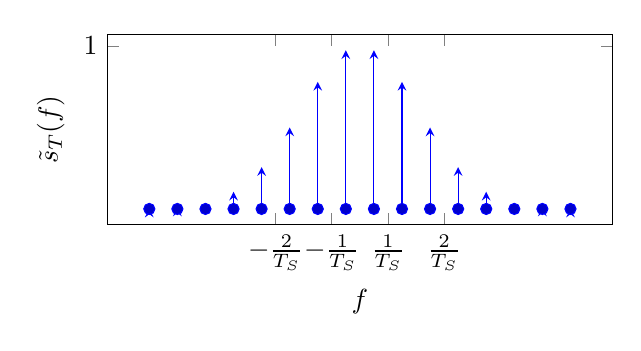
\begin{tikzpicture}
\begin{axis}[width=8cm,height=4cm,black,xlabel=$f$,ylabel=$\tilde{s}_T(f)$,ytick={1},xtick={-1,-.334,.334,1},xticklabels={$-\frac{2}{T_S}$,$-\frac{1}{T_S}$,$\frac{1}{T_S}$,$\frac{2}{T_S}$}]
\addplot+ [quiver={u=0,v=exp(-x*x)},-stealth,samples=16,domain=-2.5:2.5] {0};
\end{axis}
\end{tikzpicture}
\label{fig:inviluppo_modulazione_angolare}}\quad\subfloat[Spettro segnale modulato]{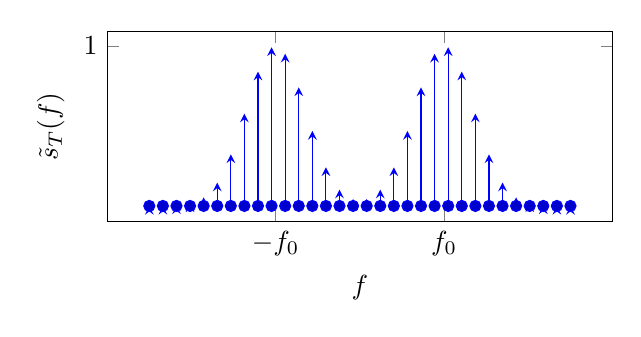
\begin{tikzpicture}
\begin{axis}[width=8cm,height=4cm,black,xlabel=$f$,ylabel=$\tilde{s}_T(f)$,ytick={1},xtick={-2,2},xticklabels={$-f_0$,$f_0$}]
\addplot+ [quiver={u=0,v=exp(-(x-2)^2)+exp(-(x+2)^2)},-stealth,samples=32,domain=-5:5] {0};
\end{axis}
\end{tikzpicture}}
\end{figure}

Lo spettro a righe del segnale modulato ha infiniti contributi ma dal punto di vista ingegneristico sono rilevanti i contributi alla potenza di un insieme finito di righe.
La banda di frequenze di interesse è definita secondo la regola o \keyword[principio!di Carson]{principio di Carson} in funzione della frequenza del tono modulante $f_s$ e la deviazione di frequenza di picco:
\begin{equation}B_T\cong 2f_s+2\Delta f_p\label{eq:Carson}\end{equation}
Nel caso non si utilizzi un tono sinusoidale ma un generico segnale portante con banda $B$ la regola diventa
\begin{equation}B_T\cong 2B+2\Delta f_p\label{eq:Carson_generico}\end{equation}
Nel dimensionamento si cercherà la minore deviazione di frequenza di picco $\Delta f_p$ per non eccedere nella banda $B_T$. Se $\frac{\Delta f_p}{B}\ll 1\implies B_T\cong 2B$.

\section{Calcolo del rapporto \ac{SNR}}
Nel canale di trasmissione passa banda al segnale modulato angolarmente si somma un segnale di disturbo descritto da un rumore bianco gaussiano a banda stretta, per cui all'ingresso del ricevitore al demodulatore si ha il segnale ricevuto:
\begin{equation}
s_R(t)=A\cos{\omega_0 t+\phi(t)}+N(t)
\end{equation}
Il rumore $N(t)$ sovrapposto alla portante in ricezione può essere scomposto nelle sue componenti in fase e quadratura rispetto alla portante $\cos{\omega_0 t}$:
\begin{equation}
s_R(t)=A\cos{\omega_0 t+\phi(t)}+n_I(t)\cos{\omega_0 t}-n_Q(t)\sen{\omega_0 t}
\end{equation}
dove il rumore espresso con forma fasoriale:
\begin{equation}
N(t)=\rho(t)\cos{\omega_0 t+\phi_N(t)}\quad\begin{cases}
\rho(t)=\sqrt{n_I^2(t)+n_Q^2(t)}\\\phi_N(t)=\arctan\frac{n_I(t)}{n_Q(t)}\end{cases}
\end{equation}

Essendo le componenti del rumore $n_I$ e $n_Q$ due gaussiane ho che l'ampiezza del rumore $\rho(t)$ è descritto da una variabile aleatoria di Rayleigh.
Si ha inoltre che il rumore sulla fase $\phi_N(t)$ è una variabile aleatoria con distribuzione continua uniforme costante in $[0,2\pi]$.

Il segnale ricevuto si può esprimere pertanto come somma dei contributi
\begin{equation}
s_R(t)=\Re{A\e{\jmath\omega_0 t}\e{\jmath\phi (t)}+\rho(t)\e{\jmath\phi_N(t)}\e{\jmath\omega_0 t}}=\Re{R\e{\jmath(\omega_0 t+\phi (t)+\beta(t))}}
\end{equation}
\begin{figure}[!ht]\centering
\begin{tikzpicture}[>=latex',black,scale=.9]
\draw[<->](0,4)node[above]{$\Imaginarypart$}--(0,0)--(6,0)node[right]{$\Realpart$};
\coordinate (A) at ($(30:5)$);
\coordinate (B) at ($(A)+(90:1)$);
\draw[thick,->](0,0)--node[below]{$A$}(A);
\draw[thick,->](0,0)--node[above]{$R$}(B);
\draw[gray](A)--+(120:.86) (A)--+(30:.5);
\draw[thick,->](A)--node[pos=1,above right]{$\rho(t)$}(B);
\node[draw,cloud,cloud puffs=15,minimum width=2cm,minimum height=2cm]at(A){};
\draw[double](1,0) arc(0:30:1)node[pos=.5,right]{\footnotesize$\omega_0 t$};
\draw($(A)+(0,.3)$) arc(90:120:.3)node[pos=.5,above]{\footnotesize$\beta$};
\draw(30:1) arc(30:40:1)node[pos=.75,right]{\footnotesize$\beta(t)$};
\draw[double]($(A)+(30:.3)$) arc(30:90:.3)node[pos=.5,right]{\footnotesize{$\phi_N(t)-\phi(t)$}};
\end{tikzpicture}
\caption{Segnale modulato angolarmente affetto da rumore gaussiano con $\rho\ll 1$}\label{fig:segnale_modulato_angolarmente_affetto_da_rumore}
\end{figure}

La deviazione di fase $\beta(t)$ è data dalla componente del rumore in quadratura $n_Q(t)$ e il modulo del segnale modulato angolarmente sarà approssimativamente sempre di ampiezza $A$ se il segnale rumore ha modulo $\rho(t)\ll 1$ essendo:
\[\sen{\beta(t)}\cong\beta(t)\cong\frac{\rho\sen{\phi_N(t)-\phi(t)}}{A}=\frac{\rho\sen{\phi_N(t)}}{A}=\frac{n_Q(t)}{A}\]
Tale deviazione assume le caratteristiche statistiche del rumore in quadratura ovvero una distribuzione uniforme in $[0,2\pi]$.

In definitiva si è trasmesso un segnale modulato angolarmente con fase $\phi(t)$ e si ha un segnale ricevuto con fase $\phi(t)+\beta(t)=\phi(t)+\tfrac{n_Q(t)}{A}$ quando il sistema lavora “\emph{sopra soglia}” ovvero con una potenza del segnale portante $A^2/2$ sufficientemente grande in rapporto alla potenza del segnale rumore.
\begin{equation}\begin{split}
P_S&=\lim\limits_{n\to\infty}{\frac{1}{2 n T}\intd{-n T}{n T}{A^2(t)\cos[2]{\omega_0 t}}{t}}=\\
&=\lim\limits_{n\to\infty}{\frac{1}{2 n T}\intd{-n T}{n T}{\frac{A^2(t)}{2}\left[1+\cos{2\omega_0 t}\right]}{t}}=\frac{P_A}{2}
\end{split}\end{equation}

Il rapporto segnale rumore dopo il demodulatore espresso come rapporto tra la potenza picco-picco del segnale e la potenza media del segnale rumore valutata in uscita dal demodulatore calcolata sulla densità spettrale bilatera del rumore in uscita dal canale di trasmissione $h_n=\frac{N_0}{2}$ moltiplicata per la banda di interesse $B_T$ ottenuta con il principio di Carson:
\begin{equation}
\restrict{\frac{S}{N}}{o}=\frac{P_\text{pp}}{\frac{N_0}{2}\frac{2}{A^2}\cdot 2B_T}
\end{equation}

\section{Demodulazione FM}
Per la modulazione di frequenza in ricezione si valuta con un derivatore in cascata al demodulatore di fase la deviazione di frequenza del segnale trasmesso essendo $\Delta f(t)=\frac{1}{2\pi}\deriv{\phi(t)}{t}$. Tale deviazione di fase è affetta dal rumore sovrapposto al segnale per cui si ha
\[\Delta f(t)=\frac{1}{2\pi}\deriv{(\phi(t)+\beta(t))}{t}=\frac{1}{2\pi}\dot{\phi}(t)+\frac{1}{2\pi}\dot{\beta}(t)\]

La potenza del segnale rumore si ottiene integrando nella banda del segnale la densità spettrale di potenza di rumore all'uscita del demodulatore angolare.
Essendo la derivata del rumore di fase $h_{nu}=\frac{h_n}{P_R}f^2$, dove $P_R=A^2/2$ è la potenza del segnale ricevuto, si calcola la potenza media del rumore all'uscita
\begin{equation}
P_{N_u}=\intd{-B}{B}{\frac{h_n}{P_R}f^2}{f}=2\intd{0}{B}{\frac{N_0}{A^2}f^2}{f}=\frac{2}{3}\frac{N_0}{A^2}B^3
\end{equation}

Per il dimensionamento del sistema si può calcolare dato un richiesto rapporto \ac{SNR} imponendo che sia
\begin{equation}
\frac{A^2}{2}\gg\frac{N_0}{2}\cdot 2B_T
\end{equation}
\begin{equation}
\restrict{\frac{S}{N}}{\text{dopo demod}}=\frac{3 P(\Delta f)}{2\frac{N_0}{A^2}B^3}=\frac{\Delta f_p^2}{\frac{N_0}{\frac{A^2}{2}}\frac{B^3}{3}}=3\left(\frac{\Delta f_p}{B}\right)^2\frac{A^2/2}{N_0 B}
\end{equation}

\begin{esempio}
Se ad esempio dato un rapporto segnale rumore richiesto tale che $\frac{S}{N}\gg\num{1e4} [\SI{40}{\decibel}]$ devo risolvere il sistema per il minimo $\Delta f_P$
\[\begin{cases}
3\left(\frac{\Delta f_p}{B}\right)^2\frac{P_R}{N_0 B}\gg\num{1e4}\\\frac{P_R}{N_0 B_T}\gg 10 \iff \frac{P_R}{N_0(2B+2\Delta f)}\gg 10
\end{cases}\]

Se ad esempio $\frac{S}{N}=\SI{40}{\decibel}$, $B=\SI{15}{\kilo\hertz}$, $F=\SI{10}{\decibel}$, $\alpha=\SI{100}{\decibel}$ con la modulazione di frequenza si ottiene dividendo membro a membro:
\[\frac{3\left(\frac{\Delta f_p}{B}\right)^2\frac{P_R}{N_0 B}}{\frac{P_R}{N_0(2B+2\Delta f)}}=\frac{10^4}{10}\]
da cui si ottiene $\Delta f_p=\SI{77}{\kilo\hertz}$ e una potenza ricevuta $P_R=\SI{-101}{\decibel}$.

Rispetto alla modulazione di ampiezza \ac{DSB-SC} per cui si è calcolata la potenza ricevuta $P_R=\SI{-79}{\decibel}$ con la modulazione di frequenza si ha un risparmio di potenza a spese di un maggiore uso di banda.
\end{esempio}
\clearpage
\section{Trasmissione su canale radio}\label{cap:canale_radio_attenuazione_spazio_libero}
In alternativa ai mezzi trasmissivi basati sulle guida d'onda con effetti dissipativi è possibile realizzare sistemi di telecomunicazione basati sulla propagazione di onde irradiate nello spazio libero. Il segnale trasmesso subisce una attenuazione dovuta all'aumentare della superficie del fronte d'onda. La densità di potenza per unità di superficie diminuisce con il quadrato della distanza.

Nel caso di antenna omnidirezionale l'\keyword[attenuazione!di spazio libero]{attenuazione di spazio libero} calcolata ipotizzando l'assenza di ostacoli tra il trasmettitore $T_X$ e ricevitore $R_X$, è
\begin{equation}
\alpha_\text{SL}=\frac{4\pi R^2}{G_T A_R}
\label{eq:radio_attenuazione_spazio_libero}
\end{equation}
dove $G_T$ è il guadagno d'antenna trasmittente, $A_R$ l'area efficace d'antenna ricevente. L'area efficace di una antenna è legata al suo guadagno dalla relazione
\begin{equation}
\frac{G}{A}=\frac{4\pi}{\lambda^2}
\label{eq:radio_legame_area_efficace_guadagno_antenna}
\end{equation}

\begin{figure}[ht]\centering
	\begin{tikzpicture}
	\draw (0,3) pic{antenna} --++(0,-.5)--++(-.5,-1.5)++(.5,1.5)--++(.5,-1.5)++(-.5,0) node[below]{Tx};
	\draw (9,3) pic[rotate=180]{antennarx} --++(0,-.5)--++(-.5,-1.5)++(.5,1.5)--++(.5,-1.5)++(-.5,0)node[below]{Rx};
	\draw [dotted] (3,3)--node[above]{$R$}(6,3);
	\end{tikzpicture}
\end{figure}

L'attenuazione di spazio libero è un fenomeno deterministico che vale per frequenze $f\ll\SI{3}{\giga\hertz}$, per le quali è sufficiente considerare solo questa attenuazione causata dalla divergenza sferica; per $f>\SI{3}{\giga\hertz}$ è necessario considerare le perdite dissipative aleatorie dovute all'atmosfera.

Tale fenomeno causa un ulteriore effetto di attenuazione, esponenziale con la distanza, dovuto alle molteplici stratificazioni di gas ionizzati, paralleli alla superficie terrestre, che causano percorsi di diffrazione. Tali fenomeni consentono la comunicazione anche non in linea d'aria tra stazioni radio situate in luoghi remoti della Terra.

\begin{figure}[ht]\centering
	\begin{tikzpicture}[scale=.66]
	\draw (4,0)arc(0:180:4);
	\foreach\x in{8,7.8,7.5,6.75}
		\draw [dashed,gray](\x,0)arc(0:180:\x);
	\draw [rotate=60](0,5.5) pic[rotate=60,scale=.33]{antenna}--++(0,-.5)--++(-.5,-1)++(.5,1)--++(.5,-1)++(-.5,0)node[below]{Tx};
	\draw [rotate=-60](0,5.5) pic[rotate=120,scale=.33]{antennarx} --++(0,-.5)--++(-.5,-1)++(.5,1)--++(.5,-1)++(-.5,0)node[below]{Rx};
	\draw[rotate=90,decorate,decoration={random,amplitude=2}](60:5.5)--(30:7)--(-30:7)--(-60:5.5);
\end{tikzpicture}
\caption{Effetto degli strati di gas ionizzati in atmosfera terrestre}
\label{fig:percorsi_diffrazione_atmosfera}
\end{figure}

\clearpage
\section{Effetti dovuti a cammini multipli}\label{cap:canale_radio_effetti_cammini_multipli}
A causa delle disomogeneità dell'atmosfera le onde trasmesse si propagano dal trasmettitore al ricevitore seguendo cammini multipli. Ciascun fronte d'onda fornisce un contributo diverso in ampiezza e fase. Le ampiezze a grande distanza avranno attenuazioni simili quindi contributi comparabili mentre le fasi si presenteranno con differenze casuali che vanno descritte statisticamente.
\begin{figure}[ht]\centering
	\begin{tikzpicture}
	\draw (0,3) pic{antenna} node[below]{Tx};
	\draw (9,3) pic[rotate=180]{antennarx} node[below]{Rx};
	\foreach\i in{-15mm,-10mm,-5mm,0,5mm,10mm,15mm}
		\draw [dotted,decorate,decoration={bent,amplitude=\i}] (1,3)--(8,3);
	\end{tikzpicture}
	\caption{Rappresentazione di cammini multipli}
	\label{fig:cammini_multipli}
\end{figure}

Il segnale ricevuto $s_R(t)$ sarà somma di tanti contributi indipendenti le cui componenti in fase e quadratura hanno distribuzione gaussiana normale, $\begin{array}{c}X\\Y\end{array}\sim\mathcal{N}(0,\sigma^2)$:

\begin{equation}
s_R(t)=x(t)\cos{\omega_0 t}-y(t)\sen{\omega_0 t}=R\cos{\omega_0 t+\phi(t)}=\Re{R\e{\imath\omega_0 t}\e{\imath\phi(t)}}
\end{equation}

L'ampiezza del segnale risultante dato dalla combinazione delle due variabili gaussiane incorrelate assume le caratteristiche statistiche di una variabile aleatoria di Rayleigh $R=\sqrt{X^2+Y^2}$ con funzione densità di probabilità \[f_R(r)=\frac{r}{\sigma^2}\e{-\frac{r^2}{2\sigma^2}}\]
\begin{figure}[ht!]\centering
	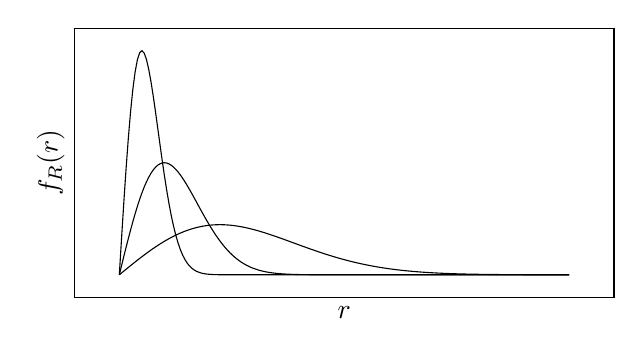
\begin{tikzpicture}
	\begin{axis}[yscale=0.6,xlabel=$r$,ylabel=$f_R(r)$,xtick=\empty,ytick=\empty]
	\foreach\var in{.25,1.0,5.0} {
		\addplot[domain=0:10,samples=200]{x/\var*exp(-x^2/(2*\var))};
%		\node[pin=45:{$\sigma=\var$}] at(0,0){}; %at(1,\eval{exp(-1/(2*\var))/\var})
	}
	\end{axis}
	\end{tikzpicture}
	\caption{Funzione densità di probabilità di Rayleigh ($\sigma^2=\{1/4,1,5\}$)}
	\label{fig:funz_dens_prob_rayleigh}
\end{figure}

La probabilità che la sovrapposizione delle onde dovuta a cammini multipli causi un \keyword[probabilità!di fuori servizio]{fuori servizio} coincide con la probabilità che l'ampiezza del segnale risultante sia inferiore ad una soglia ovvero che la potenza picco-picco del segnale ricevuto sia inferiore alla \keyword[potenza!di fuori servizio]{potenza di fuori servizio} $P_\text{FS}$:
\begin{equation}
\P{P_R^\text{pp}<P_\text{FS}}=1-\e{-\frac{h_s}{2\sigma^2}}
\label{eq:probabilita_fuori_servizio}
\end{equation}

La potenza di picco del segnale $s_R(t)$ è una variabile aleatoria esponenziale con \[R^2=\E{R^2}=\E{X^2+Y^2}=\sigma^2+\sigma^2=2\sigma^2\]

\clearpage
\section{Modello ad echi}\label{cap:canale_radio_modello_ad_echi}
Il fenomeno fisico dei cammini multipli può essere schematizzato come un sistema che somma un segnale ricevuto da un percorso diretto più lo stesso segnale ritardato. Il sistema può essere generalizzato alla somma di più echi.
\begin{figure}[h!]
\centering
	\begin{tikzpicture}[>=latex',thick,start chain=going right,node distance=1cm,every node/.style={on chain},every join/.style={->},block/.style={draw,align=center}]
	\node[join](sT) {$s_T(t)$};
	\coordinate[on chain,join](n);
	\draw[join,fill](n) circle(2pt);
	\begin{scope}[start branch=right]
	\coordinate[on chain=going below](n2);
	\node[block,join,minimum width=15mm](r){$a\e{\imath\omega\tau}$};
	\end{scope}
	\node[sum,join,right=3cm of n](s) {$+$};
	\draw[->](r)-|(s);
	\draw(n)--(n2);
	\node[join,right=of s](sR) {$s_R(t)$};
	\end{tikzpicture}
\caption{Modello sistema ad eco}
\label{fig:sistema_con_ritardo}
\end{figure}

La funzione di trasferimento del sistema per la sovrapposizione di un segnale con il suo eco:
\begin{equation}\begin{split}
H(\omega)&=1+a\e{-\jmath\omega\tau}\\
\abs{H(\omega)}&=\sqrt{(1+a\cos{\omega\tau})^2+a^2\sen[2]{\omega\tau}}=\\&=\sqrt{1+a^2+2a\cos{\omega\tau}}
\end{split}\end{equation}
Tale funzione presenta i massimi per le frequenze che si sommano costruttivamente al nodo sommatore ovvero per le quali il ritardo $\tau$ corrisponde ad uno sfasamento di multipli di $2\pi$. Nel caso di più ritardi i massimi e minimi della funzione di trasferimento possono presentarsi in modo periodico se i ritardi sono in rapporto armonico.
\begin{figure}[!ht]\centering
\begin{tikzpicture}\def\a{3.0}
\begin{axis}[xlabel=$\omega\tau$,yscale=0.5,ylabel=$\abs{H(\omega)}$,xtick={3.1415,6.2832},ytick={4,16},yticklabels={$1-a$,$1+a$},xticklabels={$\pi$,$2\pi$},extra x ticks={1},extra x tick labels={$B$},extra x tick style={grid=major}]
\addplot[domain=0:6.28,smooth] {sqrt{1+\a^2+2*\a*cos((x))}};
\end{axis}
\end{tikzpicture}
\caption{Diagramma funzione di trasferimento per modello ad echi con attenuazione $a$ e ritardo $\tau$}
\label{fig:ritardo_echi}
\end{figure}

Si può approssimativamente considerare $\abs{H(\omega)}$ costante per $B\ll\frac{1}{\tau}$. Nel caso di echi multipli si deve avere $B\ll\frac{1}{\tau_\text{max}}$. Se la banda non è piccola rispetto all'inverso del massimo ritardo il modello non è valido.


\section{Diversità spaziale e di frequenza}
Per ridurre la probabilità di fuori servizio dovuto ai cammini multipli e al modello ad echi è possibile utilizzare il concetto di \keyword[cammini multipli!diversità spaziale]{diversità spaziale} in ricezione per aumentare l'affidabilità di un ponte radio senza aumentare la potenza trasmessa. La soluzione ha il costo di porre una seconda antenna in ricezione posta ad una certa distanza dalla prima antenna ricevente e di selezionare in ricezione il segnale captato che ha subito minore attenuazione per sfasamento. La probabilità che si verifichi una attenuazione tale da causare il fuori servizio su entrambe le antenne è necessariamente minore: $P_\text{FS}^\text{Tot}=P_\text{FS}\cdot P_\text{FS}$.

Una alternativa alla trasmissione con un cammino radioelettrico differente tra antenne è possibile ottenere il risultato trasmettendo lo stesso segnale su due portanti a frequenza differente, che avranno attenuazione massima diversa per la \keyword[cammini multipli!diversità in frequenza]{diversità in frequenza} e selezionando in ricezione il segnale più potente. Tale tecnica richiede più banda ma si ha il risparmio di non dover installare più antenne.
